\subsection{Kanban}

Kanban ist eine agile Methode zur Steuerung von Softwareentwicklungsprozessen. Bei der Kanban Methode wird ein Kanban-Board verwendet, dies kann entweder ein Whiteboard sein oder digital abgebildet werden (z.B. Trello, Microsoft Teams To-Do). Bei Kanban werden die einzelnen Arbeitspakete als Karten dargestellt und in verschiedene Kategorieren eingeteilt. Im bereich der Softwareentwicklung könnten zum beispiel die Kategorien Anforderungen, Programmierung, Dokumentation, Test und Inbetriebnahme verwendet werden. Einzelne Arbeitspakete können in vielen Fällen direkt vom Projektstrukturplan übernommen werden, werden in manchen Fällen aber noch genauer spezifiziert und aufgeteilt. \cite{kanban_vorgehensmodell}

Das Projektteam hat ursprünglich das Kanban System von Microsoft Teams verwendet, jedoch hat sich zeitlich herausgestellt, dass dieses nicht so benutzerfreundlich und flexibel ist wie Trello. Aus diesem Grund hat sich das Projektteam entschieden auf Trello zu wechseln. Trello wurde verwendet um die schriftliche Arbeit einzuteilen und zu organisieren. Für diesen Zweck hat sich das Projektteam auf folgende Kategorien geeinigt:
\begin{itemize}
  \item To-Do: Hier werden die Aufgaben aufgelistet, die noch erledigt werden müssen.
  \item In Progress: Hier werden die Aufgaben aufgelistet, die gerade bearbeitet werden.
  \item Done: Hier werden die Aufgaben aufgelistet, die bereits erledigt wurden.
\end{itemize}

\begin{figure}[!ht]
  \centering
  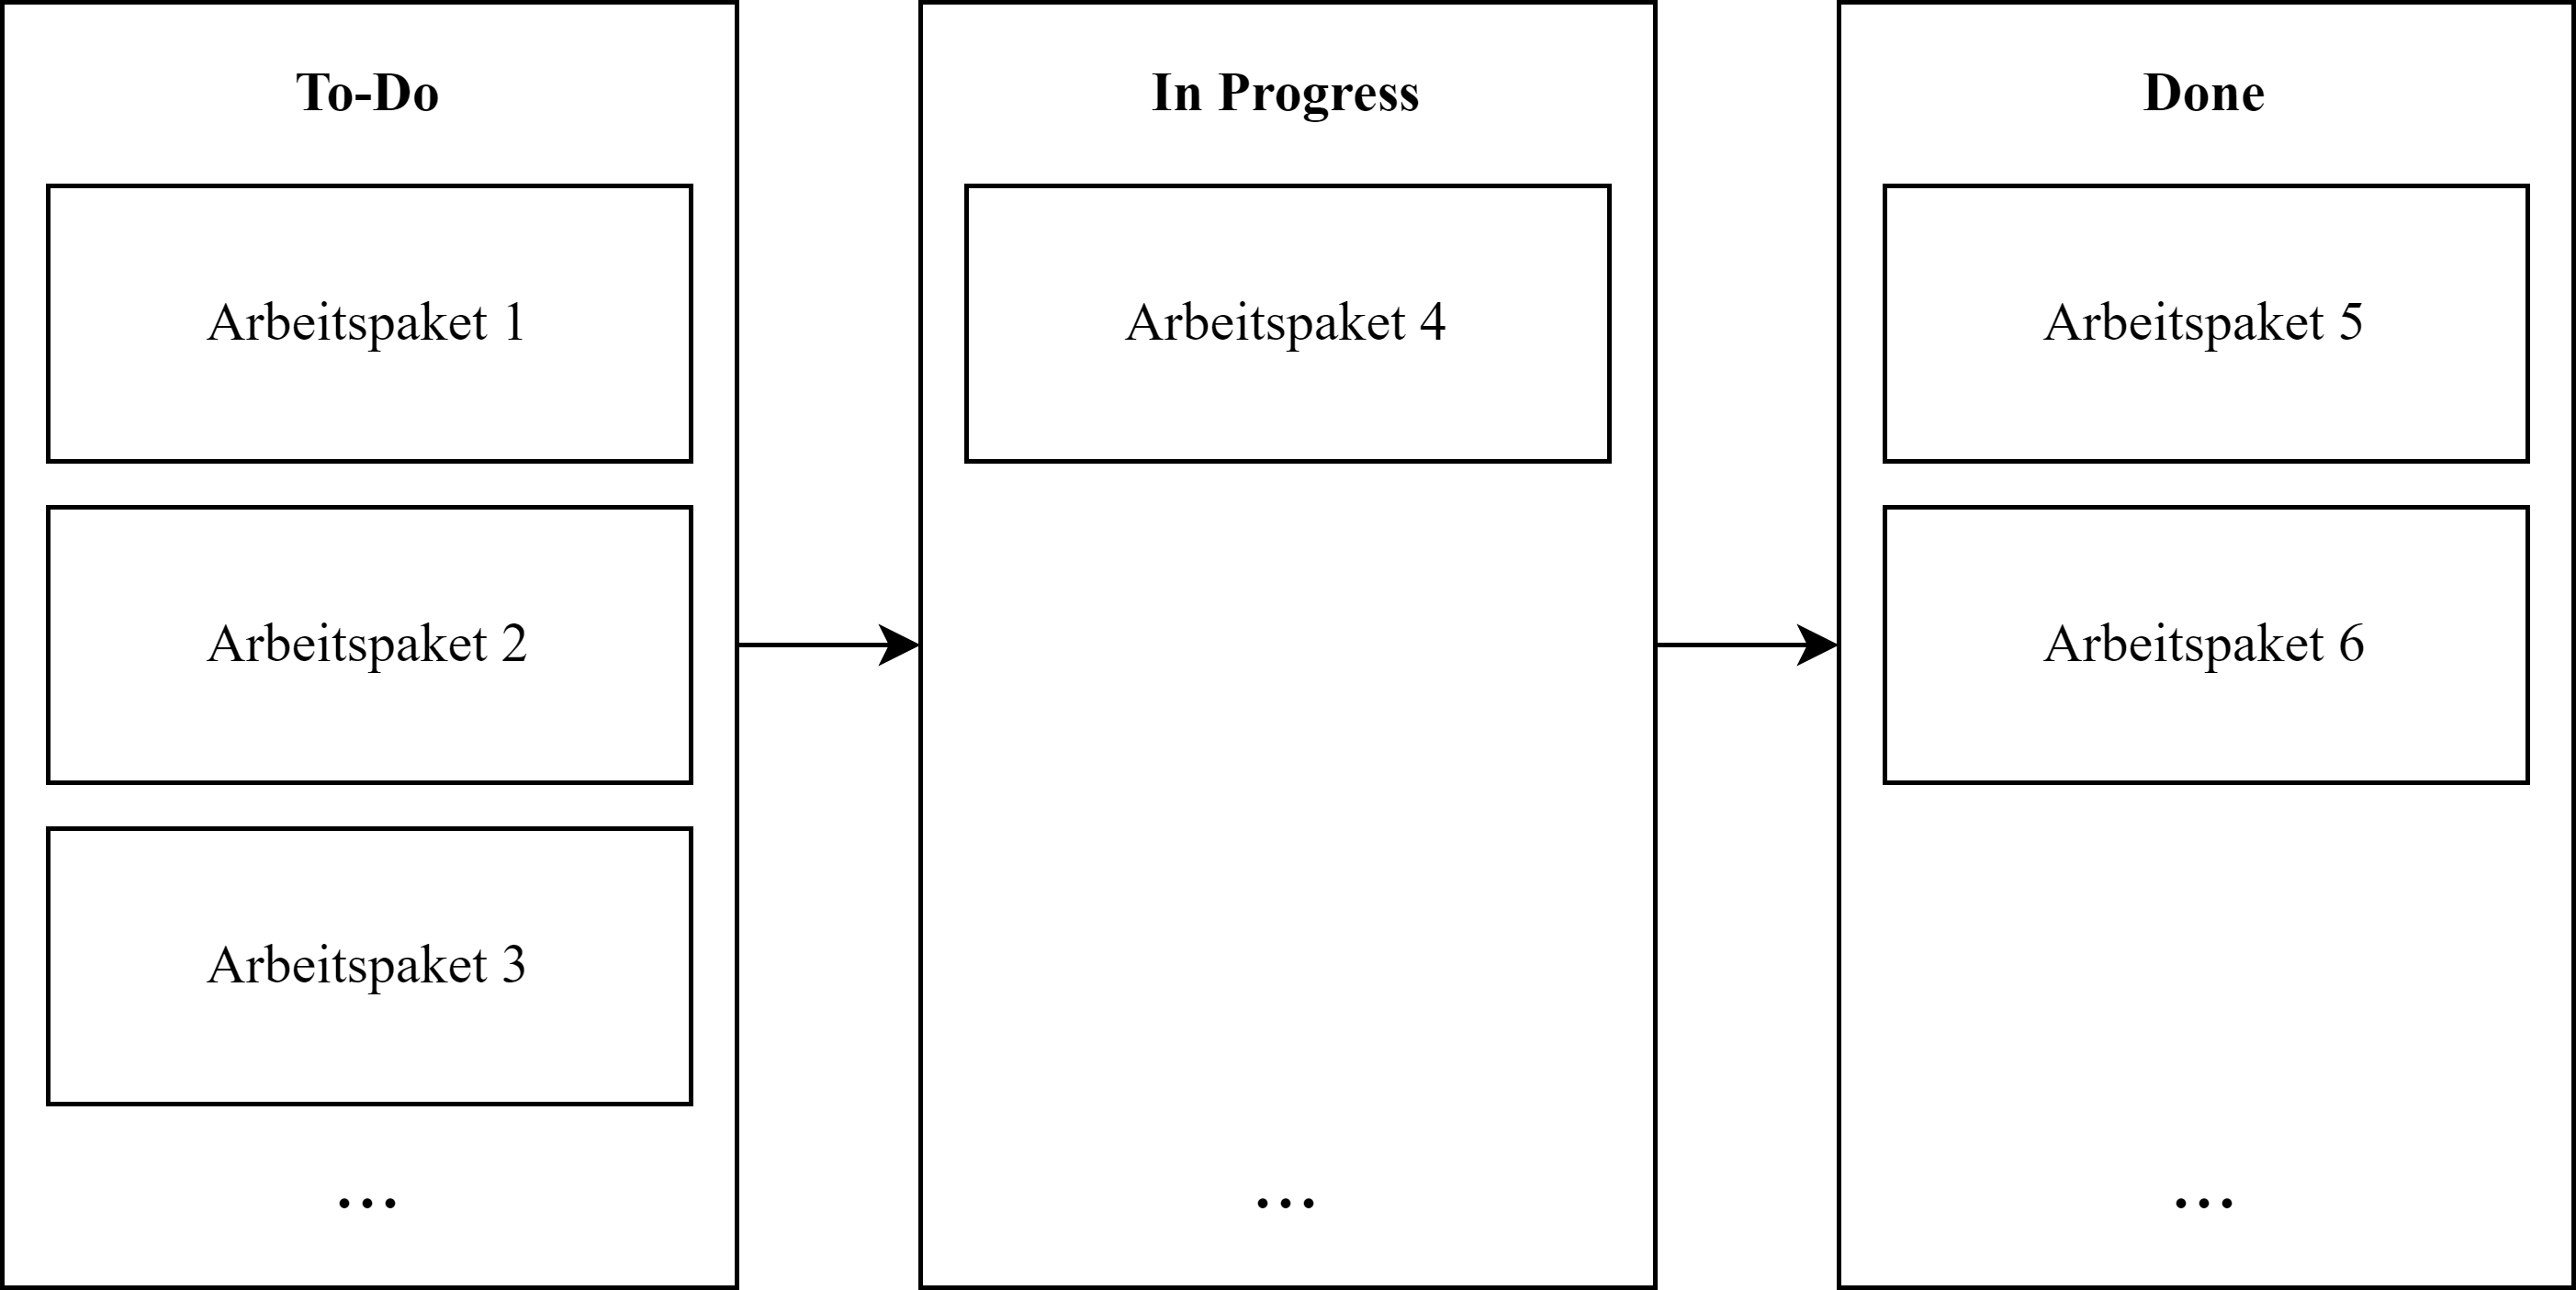
\includegraphics[width=0.8\textwidth]{images/kanban.png}
  \caption{Schematische Darstellung eines Kanban-Boards}
  \label{fig:kanban}
\end{figure}

